\section{Protocol Overview}
\label{chp:case-study}
As a case study, we focus on a standard simplified asset transfer process from Alice on chain $C_A$ to Bob on chain $C_B$ through a liquid provider in $C_A$ and $C_B$ \cite{introdefi}. 

%\begin{figure*}[!ht]
%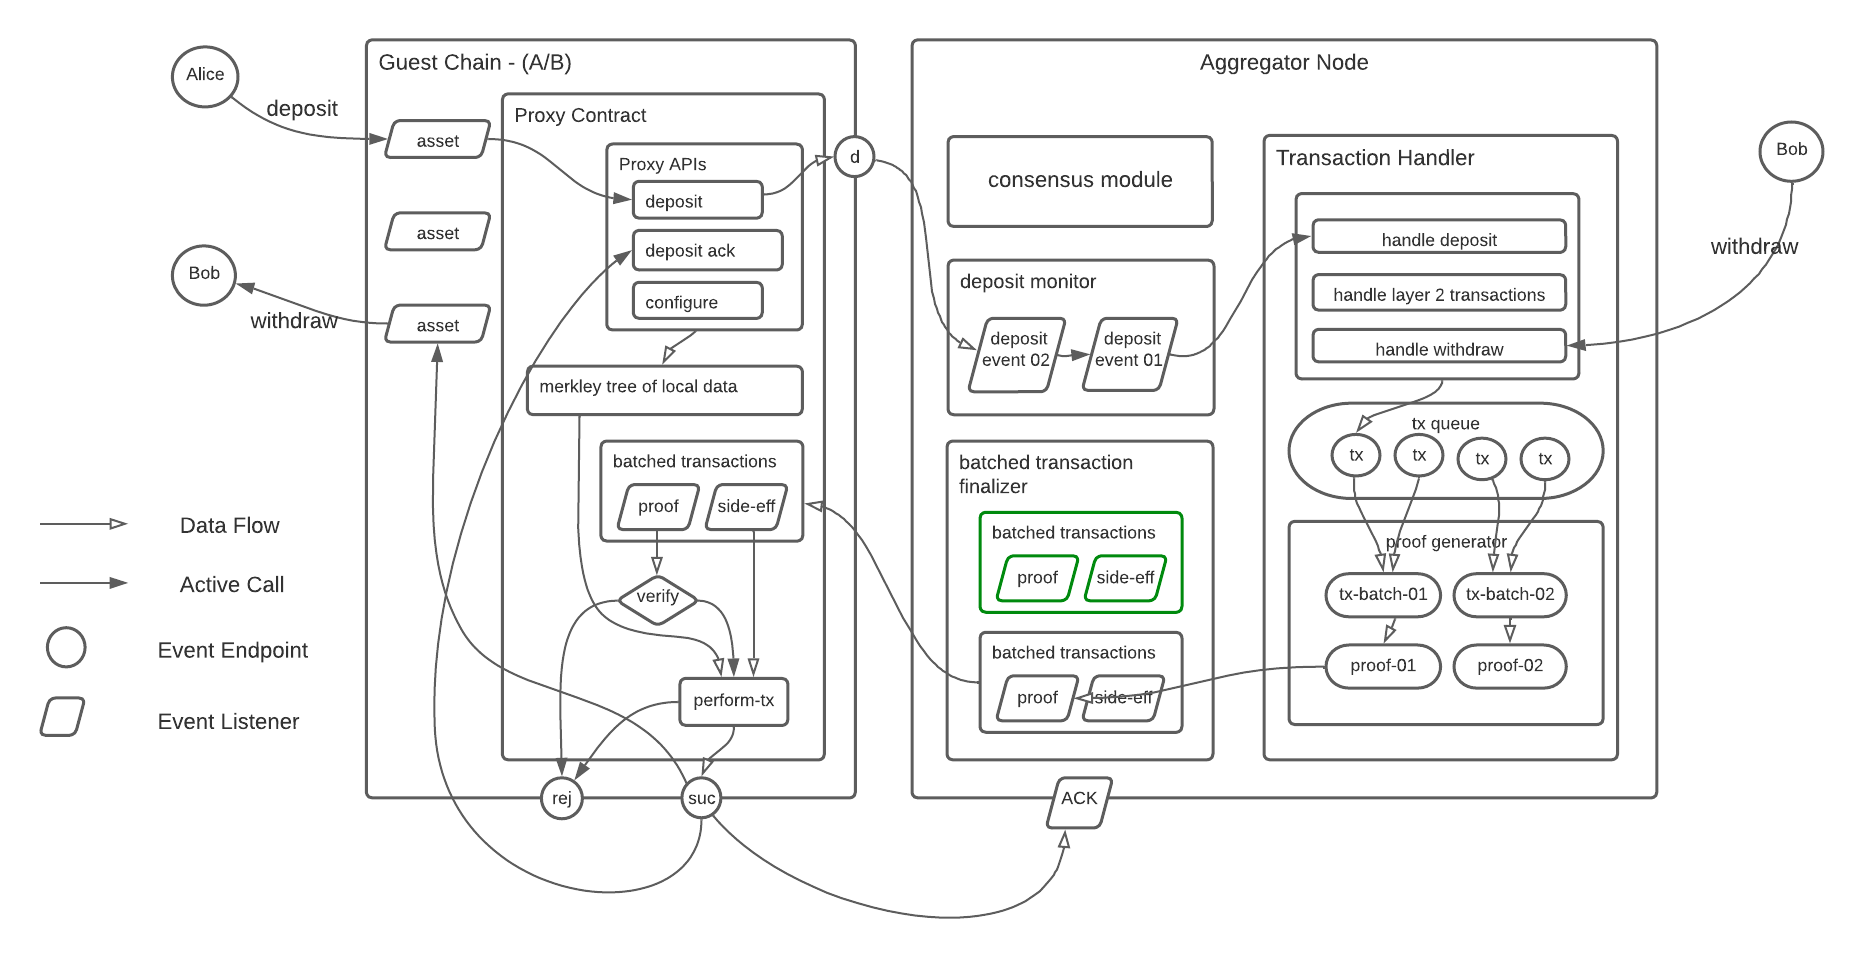
\includegraphics[scale=0.6]{case-study}
%\caption{Case study of a cross-chain token transfer}
%\label{case-study}

%\end{figure*}

\subsection{State Abstraction}
First, 
%we define the native-chain set in the bundled transfer transaction to be $\mathbb{C} = \left\{C_A, C_B\right\}$. As Alice has some assets on $C_A$ and Bob has some assets on $C_B$ and a liquid provide has assets both on $C_A$ and $C_B$, 
we can abstract our local state $s_A$ of $C_A$ and $s_B$ of $C_B$ separately as follows.

\begin{lstlisting}[escapeinside={(*}{*)}, basicstyle=\small, xleftmargin=0.6cm, backgroundcolor = \color{lightgray}, numbers=left]
(*$s_A$*) = state {
    alice: number
    lp: number
}
(*$s_B$*) = state {
    bob: number
    lp: number
}
\end{lstlisting}

Now, as we described in Section \ref{prelimiary}, the underlying global state $s$ of transfer is a tuple of $C_A$ and $C_B$:
\begin{lstlisting}[escapeinside={(*}{*)}, basicstyle=\small, xleftmargin=0.6cm, backgroundcolor = \color{lightgray}, numbers=left]
s = state {
    sa: (*$s_A$*),
    sb: (*$s_B$*)
}
\end{lstlisting}
Second, the bundled transfer transaction $tx$ can be defined as a function on global state $s$ as follows:
\begin{lstlisting}[escapeinside={(*}{*)}, xleftmargin=0.6cm, basicstyle=\small, backgroundcolor = \color{lightgray}, numbers=left]
function transfer(amount) {
  transfer(Alice, amount, lp);
  
  s.sa.alice = s.sa.alice - amount;
  s.sa.lp = s.sa.lp + amount;
  
  s.sb.bob = s.sb.bob + amount;
  s.sb.lp -= amount;
  
  if(s.sb.lp > amount) {
    transfer(lp, amount, Bob);
  }
}
\end{lstlisting}
where line 2 can be treated as the invoke transaction on $C_A$, line 4-12 are bundled transactions that will be simulated on the aggregator layer and line 11 is the side effect on $C_B$.

Unlike other bridge-like solutions which performs 2-5 on $C_A$, 7-11 on $C_B$, and using relayers to synchronize two parts, \dprotocol simulates the transaction in the aggregator chain on global state $s$ and then uses ZKP of the simulation to convince native block chains to update their local states.

We divide the life cycle of the transfer transaction into four stages: consensus stage, operating state, proving stage and finalizing stage
%(see Figure \ref{case-study}).



\smallskip\noindent\emph{Consensus Stage.}
A user Alice transfers a certain amount of money into a proxy contract (line 2). After the contract handles the invoke transaction, it commits the amount into its table of unfinalized invoke transactions and emits an event. This emitted event will get monitored by \dprotocol Node and triggers the consensus stage.

In the consensus stage, a node who wins the voting protocol generates two ZK proofs. One proves that the event is real and the other proves that the winner is picked by the consensus algorithm. (This can prevents a node systematically ignore transactions it does not want to handle). Also, Alice is allowed to withdraw the unfinalized amount after a certain amount of time (based on blockheight) (see Section \ref{chp:protocol-details} for more information about encoding consensus into ZKP circuits).

\smallskip\noindent\emph{Simulating stage:}
Once a transaction is ready to execute, it will be simulated by the voted aggregator chain node so that a new resulting global state $s'$ can be calculated from the initial state $s$. Recall that $s$ is get by aggregating states $s_i$ from different native blockchain $C_i$. It follows that by projecting $s’$ back onto different partial states, we know how to update the local state $s_A$ and $s_B$ on $C_A$ and $C_B$ accordingly.

\smallskip\noindent\emph{Proving stage:}
After the \dprotocol node finishes simulating the execution of our particular transfer transaction, it will create a zero-knowledge proof to show how to update all the partial states on $C_A$  and $C_B$.

Compared to traditional side-chain solutions, which require audit nodes to validate transactions and may suffer from majority attacks, \dprotocol uses ZKP to enforce that the simulation is carried out on predefined functions (in this case, line 4-12 in transfer transaction). Thus even the majority of the audit nodes are hacked, they can only perform attacks that lead to deny-of-service of some of the transactions. Later in Section 4 we will prove that the DOS attack is theoretically infeasible once we have a permissionless aggregator chain and any node of it can helping executing and finalizing bundled transactions if it can provide ZKP for the simulation.

Once the $tx$ was fully performed, the aggregator chain will broadcast this transaction together with its proof to native-chain $C_A$ and $C_B$.

\smallskip\noindent\emph{Finalizing Stage}:
After a zero-knowledge proof, a simulation of our transfer is generated, and the voted aggregator node will call a special finalizing contract on the native blockchains $C_A$ and $C_B$ which will verify the proof and then perform the side-effects of each sub transaction accordingly.

In the case of a transfer, after the proof is verified, $C_A$ and $C_B$ will change their local state accordingly and on $C_B$, a side effect (line 11) is performed so that Bob receives the transferred assert correctly (This amount must equal to the amount transferred by Alice otherwise the zero-knowledge proof will not be valid).


%\subsection{Application of the Zero-Knowledge Proof Technique}
%For the correctness of the simulation, the verification of ZKP on verify contract makes sure that all transactions are performed under predefined functions and the resulting state is correctly calculated (Merkle root hash is pinned). Since the transfer on $C_B$ is performed at the end, it makes sure that the amount being about to withdraw is a consequence of valid transaction simulation.

%For the correctness of the deposit monitor, ZKP is used to make sure the monitored event is pined to the native-chain root hash \cite{sidechainzkp} so that the custody of transferred tokens is reported to the aggregator node honestly. 

%For the liveness and permissionless property, \dprotocol utilizes a group of nodes and they use a BFT consensus algorithm to vote the next block generator. The ZKP of the voting result is then used to convince the native blockchains that the consensus algorithm on the aggregator layer is enforced (see \ref{consensus-stage}).

%\subsection{Cost of Zero-Knowledge Proof Verification}
%Regarding the cost problem of state pinning, since \dprotocol uses batched transactions to reduce the cost of the signature check and SNARK proof check, the problems of the high cost of state pinning and signature check can be reduced to an acceptable level.